\documentclass{article}
\usepackage{graphicx}
\usepackage[margin=1.5cm]{geometry}
\usepackage{amsmath}

\begin{document}

\title{Tuesday Reading Assessment: Unit 9, Torque and Angular Momentum}
\author{Prof. Jordan C. Hanson}

\maketitle

\section{Memory Bank}

\begin{itemize}
\item $\tau = r F \sin\theta$ ... Definition of torque.
\item Torque is the angular version of force.  It is the result of a force $F$, separated from a pivot by a distance $r$, that rotates the system about the pivot.  The angle between the force $F$ and the distance $r$ is $\theta$.
\item For sytems in \textit{static equilibrium}, the net force is zero, and the net torque is zero.
\end{itemize}

\begin{figure}[ht]
\centering
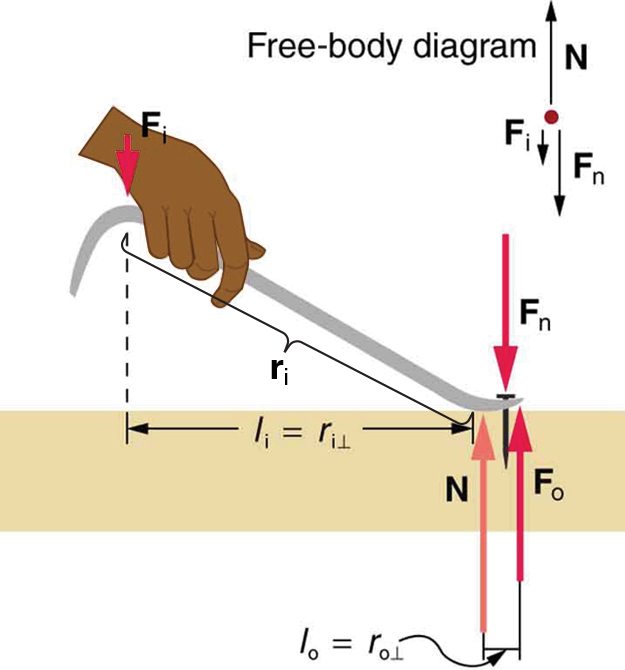
\includegraphics[width=0.25\textwidth]{figures/nail1.jpeg}
\caption{\label{fig:torque} A crowbar is used to pry a nail loose.}
\end{figure}

\section{Torque}

\begin{enumerate}
\item Suppose a doorknob is a distance of $r = 1.2$ meters from the hinges of a door.  If a force of $F = 3.0$ N is applied at an angle $\theta = 90$ degrees relative to the door, what is the torque? \\ \vspace{1cm}
\item Consider Fig. \ref{fig:torque}.  The distance $r_{1\perp}$ corresponds to the torque caused by $F_1$.  The length of the crowbar is $r_1 = 20$ cm, and it makes a 45 degree angle with the wood.  The little distance from the tool to the nail is $r_{0\perp} = l_0 = 4$ cm, and that distance corresponds to the force $F_0$.
\begin{itemize}
\item Use trigonometry to determine $r_{1\perp}$ from $r_1$ and the angle between the bar and the wood.
\item It the nail is not yet budging, this means the net torque is zero.  Set the torque on the left side of the nail ($r_{1\perp}$ and $F_1$) equal to the torque on the right-hand side ($r_{0}$ and $F_0$).  Solve algebraically for $F_0$.
\item If $F_1$ is 40 N down, what is the magnitude of $F_0$, and in what direction is it?
\item If 180 N is the forced required to pop the nail, how hard must someone push on the crowbar ($F_1$ down)?
\end{itemize}
\end{enumerate}
\end{document}
